\chapter{The way of the program}
\label{chap01}

The goal of this book is to teach you to think like a
computer scientist.  I like the way computer scientists think because
they combine some of the best features of Mathematics, Engineering,
and Natural Science.  Like mathematicians, computer scientists use formal
languages to denote ideas (specifically computations).  Like
engineers, they design things, assembling components into systems and
evaluating tradeoffs among alternatives.  Like scientists,
they observe the behavior of complex systems, form hypotheses, and test
predictions.

The single most important skill for a computer scientist is {\bf
problem-solving}.  By that I mean the ability to formulate problems,
think creatively about solutions, and express a solution clearly and
accurately.  As it turns out, the process of learning to program is an
excellent opportunity to practice problem-solving skills.  That's why
this chapter is called ``The way of the program.''

On one level, you will be learning to program, which is a useful
skill by itself.  On another level you will use programming
as a means to an end.  As we go along, that end will
become clearer.

\section{What is a programming language?}
\index{programming language}
\index{language!programming}

The programming language you will be learning is Java, which is
relatively new (Sun released the first version in May, 1995).  Java is
an example of a {\bf high-level language}; other high-level languages
you might have heard of are Python, C or C++, and Perl.

As you might infer from the name ``high-level language,'' there are
also {\bf low-level languages}, sometimes called machine
language or assembly language.  Loosely-speaking, computers can only
run programs written in low-level languages.  Thus, programs
written in a high-level language have to be translated before they can
run.  This translation takes time, which is a small disadvantage
of high-level languages.

\index{portable}
\index{high-level language}
\index{low-level language}
\index{language!high-level}
\index{language!low-level}

The advantages are enormous.  First,
it is {\em much} easier to program in a high-level language:
the program takes less time to write,
it's shorter and easier to read, and it's more likely to be
correct.  Second, high-level languages are {\bf portable},
meaning that they can run on different kinds of computers with
few or no modifications.  Low-level programs can only run
on one kind of computer, and have to be rewritten to run on
another.

Due to these advantages, almost all programs are written in
high-level languages.  Low-level languages are only used for
a few special applications.

\index{compile}
\index{interpret}

There are two ways to translate a program;
{\bf interpreting} and {\bf compiling}.  An interpreter
is a program that reads a high-level program
and does what it says.  In effect, it translates
the program line-by-line, alternately reading lines and
carrying out commands.

A compiler is a program that reads a high-level program and
translates it all at once, before running any of the commands.
Often you compile the program as a separate step, and then
run the compiled code later.  In this case, the high-level
program is called the {\bf source code}, and the translated
program is called the {\bf object code} or the {\bf executable}.

Java is both compiled and
interpreted.  Instead of translating programs into
machine language, the Java compiler generates {\bf byte code}.
Byte code is easy (and fast) to interpret, like machine language,
but it is also portable, like a high-level language.  Thus,
it is possible to compile a program on one machine,
transfer the byte code to another machine,
and then interpret the byte code on the other machine.  This
ability is an advantage of Java over many other
high-level languages.


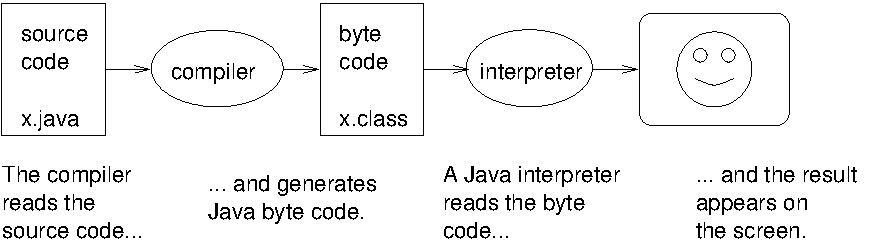
\includegraphics{figs/java.pdf}


Although this process may seem complicated, in most program
development environments these steps
are automated for you.  Usually you will only have to write a program
and press a button or type a single command to compile and run it.  On
the other hand, it is useful to know what steps are
happening in the background, so if something goes wrong you can
figure out what it is.



\section{What is a program?}

A program is a sequence of instructions that specifies how to perform
a computation\footnote{This definition does not apply to all
  programming languages; for alternatives, see
  \url{http://en.wikipedia.org/wiki/Declarative_programming}.}.  The
computation might be something mathematical, like solving a system of
equations or finding the roots of a polynomial, but it can also be a
symbolic computation, like searching and replacing text in a document
or (strangely enough) compiling a program.

\index{statement}

The instructions, which we will call {\bf statements}, look different
in different programming languages, but there are a few basic
operations most languages perform:

\begin{description}

\item[input:] Get data from the keyboard, or a file, or some
other device.

\item[output:] Display data on the screen or send data to a
file or other device.

\item[math:] Perform basic mathematical operations like addition and
multiplication.

\item[testing:] Check for certain conditions and run the
appropriate sequence of statements.

\item[repetition:] Perform some action repeatedly, usually with
some variation.

\end{description}

That's pretty much all there is to it.
Every program you've ever used, no matter how complicated, is
made up of statements that perform these operations.  Thus,
one way to describe programming is the process of breaking a
large, complex task up into smaller and smaller subtasks
until the subtasks are simple enough to be performed
with one of these basic operations.


\section{What is debugging?}
\index{debugging}
\index{bug}

For whimsical reasons,
programming errors are called {\bf bugs} and the process
of tracking them down and correcting them is called
{\bf debugging}.

There are three kinds of errors that can occur
in a program, and it is useful to distinguish them
to track them down more quickly.

\subsection{Syntax errors}
\index{syntax error}
\index{error!syntax}

The compiler can only translate a program if the program is
syntactically correct; otherwise, the compilation fails and
you will not be able to run your program.  {\bf Syntax}
refers to the structure of your program and the rules about
that structure.
\index{syntax}

For example, in English, a sentence must begin with a capital
letter and end with a period.  this sentence contains a syntax
error.  So does this one

For most readers, a few syntax errors are not a significant
problem, which is why we can read the poetry of e e cummings
without spewing error messages.

Compilers are not so forgiving.  If there is a single syntax
error anywhere in your program, the compiler will print an
error message and quit, and you will not be able to run
your program.

To make matters worse, there are more syntax rules in Java
than there are in English, and the error messages you get from
the compiler are often not very helpful.  During the first
weeks of your programming career, you will probably
spend a lot of time tracking down syntax errors.  As you
gain experience, you will make fewer errors and find
them faster.

\subsection{Run-time errors}
\label{run-time}
\index{run-time error}
\index{error!run-time}
\index{exception}
\index{safe language}
\index{language!safe}

The second type of error is a run-time error, so-called because
the error does not appear until you run the program.  In Java,
run-time errors occur when the interpreter is running the byte
code and something goes wrong.

Java tends to be a {\bf safe}
language, which means that the compiler catches a lot of errors.
So run-time errors are rare, especially
for simple programs.

In Java, run-time errors are called {\bf exceptions},
and in most environments they appear as windows or dialog
boxes that contain information about what happened and what
the program was doing when it happened.  This information is
useful for debugging.

\subsection{Logic errors and semantics}
\index{semantics}
\index{logic error}
\index{error!logic}

The third type of error is the {\bf logic} or {\bf semantic} error.
If there is a logic error in your program, it will compile and run
without generating error messages, but it will not do the right thing.
It will do something else.  Specifically, it will do what you told it
to do.

The problem is that the program you wrote is not the program you
wanted to write.  The semantics, or meaning of the program, are wrong.
Identifying logic errors can be tricky because you have to work
backwards, looking at the output of the program and trying to figure
out what it is doing.

\subsection{Experimental debugging}

One of the most important skills you will acquire in this
class is debugging.  Although debugging can be frustrating, it
is one of the most interesting, challenging, and
valuable parts of programming.

Debugging is like detective work.  You are
confronted with clues and you have to infer the processes
and events that lead to the results you see.

Debugging is also like an experimental science.  Once you have an idea
what is going wrong, you modify your program and try again.  If your
hypothesis was correct, then you can predict the result of the
modification, and you take a step closer to a working program.  If
your hypothesis was wrong, you have to come up with a new one.  As
Sherlock Holmes pointed out, ``When you have eliminated the
impossible, whatever remains, however improbable, must be the truth.''
(From A.~Conan Doyle's {\em The Sign of Four}.)

\index{Holmes, Sherlock}
\index{Doyle, Arthur Conan}

For some people, programming and debugging are the
same thing.  That is, programming is the process of gradually
debugging a program until it does what you want.  The idea
is that you should always start with a working program that
does {\em something}, and make small modifications, debugging
them as you go, so that you always have a working program.

For example, Linux is an operating system that contains thousands of
lines of code, but it started out as a simple program Linus Torvalds
used to explore the Intel 80386 chip.  According to Larry Greenfield,
``One of Linus's earlier projects was a program that would switch
between printing AAAA and BBBB.  This later evolved to Linux''
(from {\em The Linux Users' Guide} Beta Version 1).

\index{Linux}
\index{Torvalds, Linux}
\index{Greenfield, Larry}

In later chapters I make more suggestions about debugging
and other programming practices.

\section{Formal and natural languages}
\index{formal language}
\index{natural language}
\index{language!formal}
\index{language!natural}

{\bf Natural languages} are the languages that people speak,
like English, Spanish, and French.  They were not designed
by people (although people try to impose order on them);
they evolved naturally.

{\bf Formal languages} are languages designed by people for
specific applications.  For example, the notation that mathematicians
use is a formal language that is particularly good at denoting
relationships among numbers and symbols.  Chemists use a formal
language to represent the chemical structure of molecules.  And
most importantly:

\begin{quote}
{\bf Programming languages are formal languages that have been
designed to express computations.}
\end{quote}

Formal languages have strict rules
about syntax.  For example, $3+3=6$ is a syntactically correct
mathematical statement, but $3 \$ =$ is not.  Also, $H_2O$ is a
syntactically correct chemical name, but $_2Zz$ is not.

Syntax rules come in two flavors, pertaining to tokens and structure.
Tokens are the basic elements of the language, like words and numbers
and chemical elements.  One of the problems with $3 \$ =$ is that
$\$$ is not a legal token in mathematics (at least as far as I
know).  Similarly, $_2Zz$ is not legal because there is no element with
the abbreviation $Zz$.

The second type of syntax rule pertains to the structure of a
statement; that is, the way the tokens are arranged.  The statement
$3 \$ =$ is structurally illegal, because you can't have an equals
sign at the end of an equation.  Similarly, molecular formulas
have to have subscripts after the element name, not before.

When you read a sentence in English or a statement in a formal
language, you have to figure out what the structure of the sentence is
(although in a natural language you do this unconsciously).  This
process is called {\bf parsing}.

\index{parse}

Although formal and natural languages have features in
common---tokens, structure, syntax and semantics---there are
differences.

\index{ambiguity}
\index{redundancy}
\index{literalness}

\begin{description}

\item[ambiguity:] Natural languages are full of ambiguity, which
  people deal with by using contextual clues and other information.
  Formal languages are designed to be unambiguous, which means that
  any statement has exactly one meaning, regardless of context.

\item[redundancy:] To make up for ambiguity and reduce
  misunderstandings, natural languages are often redundant.  Formal
  languages are more concise.

\item[literalness:] Natural languages are full of idiom and
metaphor.  Formal languages mean exactly what they say.

\end{description}

People who grow up speaking a natural language (everyone) often have a
hard time adjusting to formal languages.  In some ways the difference
between formal and natural language is like the difference between
poetry and prose, but more so:

\index{poetry}
\index{prose}

\begin{description}

\item[Poetry:] Words are used for their sounds as well as for
their meaning, and the whole poem together creates an effect or
emotional response.  Ambiguity is common and deliberate.

\item[Prose:] The literal meaning of words is more important
and the structure contributes more meaning.

\item[Programs:] The meaning of a computer program is unambiguous
and literal, and can be understood entirely by analysis of the
tokens and structure.

\end{description}

Here are some suggestions for reading programs (and other formal
languages).  First, remember that formal languages are much more dense
than natural languages, so it takes longer to read them.  Also, the
structure is important, so it is usually not a good idea to read
from top to bottom, left to right.  Instead, learn to parse the
program in your head, identifying the tokens and interpreting the
structure.  Finally, remember that the details matter.  Little things
like spelling errors and bad punctuation, which you can get away
with in natural languages, can make a big difference in a formal
language.

\section{The first program}
\label{hello}
\index{hello world}

Traditionally the first program people write in a new language
is called ``hello world'' because all it does is display the
words ``Hello, World.''  In Java, this program looks like:

\begin{lstlisting}
class Hello {

  // main: generate some simple output

  public static void main(String[] args) {
    System.out.println("Hello, world.");
  }
}
\end{lstlisting}
%
This program includes features that are hard to explain to
beginners, but it provides a preview of topics we
will see in detail later.

Java programs are made up of {\bf class definitions}, which have
the form:

\index{class definition}
\index{definition!class}

\begin{lstlisting}
class CLASSNAME {

  public static void main (String[] args) {
    STATEMENTS
  }
}
\end{lstlisting}
%
Here {\tt CLASSNAME} indicates a name chosen by the programmer.
The class name in the example is {\tt Hello}.

\index{class!name}
\index{public}
\index{static}

{\tt main} is a {\bf method}, which is a named collection of
statements.  The name {\tt main} is special; it marks the place in the
program where execution begins.  When the program runs, it starts at
the first statement in {\tt main} and ends when it finishes the last
statement.

\index{method}
\index{print}
\index{statement!print}

{\tt main} can have any number of statements, but the example has one.
It is a {\bf print statement}, meaning that it displays a message on
the screen.  Confusingly, ``print'' can mean ``display something on
the screen,'' or ``send something to the printer.''  In this book I
won't say much about sending things to the printer; we'll do all our
printing on the screen.  The print statement ends with a semi-colon
({\tt ;}).

{\tt System.out.println} is a method provided by one of Java's
libraries.  A {\bf library} is a collection of class and method
definitions.
\index{library}

Java uses squiggly-braces (\{ and \}) to group things together.  The
outermost squiggly-braces (lines 1 and 8) contain the class
definition, and the inner braces contain the definition of {\tt main}.

\index{braces, squiggly}
\index{squiggly braces}
\index{comment}
\index{statement!comment}

Line 3 begins with {\tt //}.  That means it's
a {\bf comment}, which is a bit of
English text that you can put a program,
usually to explain what it does.  When the compiler
sees {\tt //}, it ignores everything from there until the end
of the line.


\section{Glossary}

\begin{description}

\item[problem-solving:]  The process of formulating a problem, finding
a solution, and expressing the solution.

\item[high-level language:]  A programming language like Java that
is designed to be easy for humans to read and write.

\item[low-level language:]  A programming language that is designed
to be easy for a computer to run.  Also called ``machine
language'' or ``assembly language.''

\item[formal language:]  Any of the languages people have designed
for specific purposes, like representing mathematical ideas or
computer programs.  All programming languages are formal languages.

\item[natural language:]  Any of the languages people speak that
have evolved naturally.

\item[portability:]  A property of a program that can run on more
than one kind of computer.

\item[interpret:]  To run a program in a high-level language
by translating it one line at a time.

\item[compile:]  To translate a program in a high-level language
into a low-level language, all at once, in preparation for later
execution.

\item[source code:]  A program in a high-level language, before
being compiled.

\item[object code:]  The output of the compiler, after translating
the program.

\item[executable:]  Another name for object code that is ready
to run.

\item[byte code:]  A special kind of object code used for Java
programs.  Byte code is similar to a low-level language, but it is
portable, like a high-level language.

\item[statement:] A part of a program that specifies a computation.

\item[print statement:] A statement that causes output to be displayed
  on the screen.

\item[comment:] A part of a program that contains information
about the program, but that has no effect when the program runs.

\item[method:] A named collection of statements.

\item[library:] A collection of class and method definitions.

\item[bug:]  An error in a program.

\item[syntax:]  The structure of a program.

\item[semantics:]  The meaning of a program.

\item[parse:]  To examine a program and analyze the syntactic structure.

\item[syntax error:]  An error in a program that makes it impossible
to parse (and therefore impossible to compile).

\item[exception:]  An error in a program that makes it fail at
run-time.  Also called a run-time error.

\item[logic error:]  An error in a program that makes it do something
other than what the programmer intended.

\item[debugging:]  The process of finding and removing any of
the three kinds of errors.

\index{problem-solving}
\index{high-level language}
\index{low-level language}
\index{formal language}
\index{natural language}
\index{interpret}
\index{compile}
\index{syntax}
\index{semantics}
\index{parse}
\index{exception}
\index{error}
\index{debugging}
\index{statement}
\index{comment}

\end{description}

\section{Exercises}

\begin{exercise}

Computer scientists have the annoying habit of using common
English words to mean something other than their common
English meaning.  For example, in English, statements and
comments are the same thing, but in programs they are different.

The glossary at the end of each chapter is intended to highlight
words and phrases that have special meanings in computer science.
When you see familiar words, don't assume that you know what
they mean!

\begin{enumerate}

\item In computer jargon, what's the difference between a statement
and a comment?

\item What does it mean to say that a program is portable?

\item What is an executable?

\end{enumerate}

\end{exercise}

\begin{exercise}

Before you do anything else, find out how to compile and run a Java
program in your environment.  Some environments provide sample programs
similar to the example in Section~\ref{hello}.

\begin{enumerate}

\item Type in the ``Hello, world'' program, then compile and run it.

\item Add a print statement that prints a second message after
the ``Hello, world!''.  Something witty like, ``How are you?''
Compile and run the program again.

\item Add a comment to the program (anywhere), recompile, and run
it again.  The new comment should not affect the result.

\end{enumerate}

This exercise may seem trivial, but it is the starting place for many
of the programs we will work with.  To debug with confidence,
you have to have confidence in your programming environment.  In some
environments, it is easy to lose track of which program is executing,
and you might find yourself trying to debug one program while you are
accidentally running another.  Adding (and changing) print statements
is a simple way to be sure that the program you are looking at is
the program you are running.

\end{exercise}


\begin{exercise}

It is a good idea to commit as many errors as you can think of,
so that you see what error messages the compiler produces.
Sometimes the compiler tells you exactly what is wrong, and all
you have to do is fix it.  But sometimes the error messages are
misleading.  You will develop a sense for when you can
trust the compiler and when you have to figure things out yourself.

\begin {enumerate}

\item Remove one of the open squiggly-braces.

\item Remove one of the close squiggly-braces.

\item Instead of {\tt main}, write {\tt mian}.

\item Remove the word {\tt static}.

\item Remove the word {\tt public}.

\item Remove the word {\tt System}.

\item Replace {\tt println} with {\tt Println}.

\item Replace {\tt println} with {\tt print}.  This one is
tricky because it is a logic error, not a syntax error.
The statement {\tt System.out.print} is legal, but it may or may
not do what you expect.

\item Delete one of the parentheses.  Add an extra one.

\end {enumerate}
\end{exercise}






